
\chapter{Grundlagen}
%Harm
%passt soweit
\section{Raspberry Pi}\label{Raspberry}
%TODO: Quellen!

Der Raspberry Pi wurde von der britischen Raspberry Pi Foundation entworfen um jungen Menschen den Erwerb von Programmier- und Hardwarekenntnissen zu
ermöglichen. Die Bezeichnung Raspberry Pi folgt der "`Tradition"' Computer nach Früchten zu benennen wie beispielsweise bei "`Apple"'. Das Pi steht für Phyton Interpreter und soll verdeutlichen, dass der Raspberry mit einem Phyton Interpreter ausgeliefert wird. Er ist ein Einplatinencomputer und für wenig Geld verfügbar. Der Raspberry Pi zeichnet sich durch frei programmierbare Schnittstellen aus, um beispielsweise Sensoren anzuschließen.(\cite{SWB-435432907})

Mittlerweile gibt es mehrere Modelle:

\begin{itemize} 
\item Pi Zero 
\item Pi Zero W
\item Pi 1 Modell A
\item Pi 1 Modell A+
\item Pi 1 Modell B
\item Pi 1 Modell B+
\item Pi 2 Modell B
\item Pi 3 Modell B 
\end{itemize}

Aufgrund der Vielzahl der mittlerweile verfügbaren Modelle konzentriert sich die genauere Beschreibung auf die Modelle "`2 Modell B"' und "`3 Modell B"':

\begin{table}[htb]
\centering
\caption{Vergleich von Raspberry Pi 2 und 3 \cite{CortexA7} \cite{CortexA57}}
\label{tab:VergleichRaspberry}
\begin{tabular}{l|l|l}
\textbf{Kriterium}                    & \textbf{Raspberry Pi 2}        					& \textbf{Raspberry Pi 3}           \\ \hline
Veröffentlichungsdatum       & Februar 2015          					& Februar 2016             \\ \hline
CPU                          & ARM Cortex-A7   								& ARM Cortex-A57           \\ \hline
CPU-Geschwindigkeit (in MHz) & 900             								& 1200                     \\ \hline
CPU-Kerne                    & 4                              & 4                        \\ \hline
Arbeitsspeicher (in MB)      & 1024                  					& 1024                     \\ \hline
USB 2.0-Anschlüsse           & 4                     					& 4                        \\ \hline
Ethernetschnittstelle        & 10/100 MBit Ethernet  					& 10/100 MBit Ethernet     \\ \hline
W-Lan                        & \multicolumn{1}{|c|}{-} 					& 802.11b/g/n (2,4 Ghz)    \\ \hline
Bluetooth                    & \multicolumn{1}{|c|}{-} 					& Bluetooth 4.1 Low Energy \\ \hline
Anzahl GPIO-Pins             & 26                    					& 26                       \\
\end{tabular}
\end{table}
 
Die Modelle Raspberry Pi 2 Modell B und Raspberry Pi 3 Modell B unterscheiden sich nur in wenigen Eigenschaften. Der Raspberry Pi 3 hat eine höher getaktete CPU, WLAN und Bluetooth.

%Jan
\section{Sprachen}
%passt soweit
\subsection{Python}\label{Python}
\textsc{Johannes Hubertz}\cite{hubertz2016softwaretests} schreibt, dass Python für alle gängigen Betriebssysteme verfügbar wäre und bei Linux-Distributionen würde es direkt mit ausgeliefert werden. Der Interpreter eigne sich für manuelle Eingaben, die direkt verarbeitet werden. Ebenfalls eigne sich dieser für die Ausführung von Dateien, die Python-Code enthalten. Eine Eigenheit von Python bestehe darin, alles als Objekt zu behandeln. Der Quelltext sei durch die besondere Einrückung mit Leerzeichen, der die wesentliche Ausführung bestimmt, einfach und gut lesbar. \\
Mit der Scriptsprache Python ist es möglich, die Sensoren des Raspberry Pi zu implementieren. Ebenso gibt es die Möglichkeit eine Datenbankschnittstelle und eine Schnittstelle für die Kommunikation unter den Raspberry Pi's zu erstellen.
%Hacken dran
\subsection{Java}\label{Java}
\textsc{Dietmar Abts} stellt in seinem Buch "'Grundkurs JAVA : von den Grundlagen bis zu Datenbank- und Netzanwendungen"' \cite{abts2015grundkurs} Java als eine universelle Programmiersprache für viele Anwendungen in der Industrie auf Client- und Serverseite dar.
Sie wird als Standard für die Entwicklung von Unternehmenssoftware, Webanwendungen, in technischen Systemen und in mobilen Anwendungen verwendet.
Ein besonderes Merkmal von Java sei die Plattformunabhängigkeit, d.h. Java Anwendungen sind ohne Portierung auf nahezu allen Rechnersystemen lauffähig. Java profitiere von den Erfahrungen mit anderen Programmiersprache wie C, C++ und Smalltalk. Wesentliche Konzepte wurden übernommen und fehleranfällige Eigenschaften wären bewusst ausgelassen worden, damit die Sprache verhältnismäßig robust und einfach sei.\\
Mit der Programmiersprache Java ist es möglich, die Sensoren des Raspberry Pi zu implementieren. Ebenso können Datenbankschnittstellen und Schnittstellen zur Kommunikation erstellt werden.

%Hacken dran
\subsection{\acf{SQL}}
Laut \textsc{Edwin Schick}\cite{schicker2017datenbanken} sei \ac{SQL} eine Zugriffsprache für den Endbenutzer. Als Schnittstelle für den Anwender dominieren inzwischen grafische Oberflächen. Für Datenbankprogrammierer habe die Sprache \ac{SQL} an Bedeutung gewonnen, insbesondere seit der ersten Normierung (SQL1 1987).\ac{SQL} sei die wichtigste Standardsprache für Datenbanken. \\
Die \ac{SQL} Datenbank soll als Speicher für Daten der Raspberry Pis dienen. Zusätzlich sollen die Daten aus der Datenbank lesbar sein.

%Hacken dran
\subsection{\acf{HTML}}
\textsc{Valentin Plenk}\cite{plenk2017angewandte} schreibt, dass \ac{HTML} eine textbasierte Auszeichnungssprache sei, die von Menschen für Menschen geschriebene Texte strukturiere. Durch den Webbrowser und Gestaltungsvorlagen wie \ac{CSS} wäre die visuelle Darstellung der Texte bestimmt. \ac{HTML} könne strukturierte Dokumente durch verschiedene Gliederungsebenen, Absätze und Tabellen erstellen. Zusätzlich biete es Möglichkeiten Hyperlinks, Bilder und andere multimediale Inhalte wiederzugeben. Die Grundlage des World Wide Webs seien \ac{HTML}-Dokumente, die durch die Webbrowser dargestellt werden. \\
Diese Auszeichnungssprache soll zur Darstellung des Projektes im Webbrowser dienen und somit die gesammelten Messdaten u.v.m. anzeigen.

%Hacken dran
\subsection{\acf{PHP}}\label{PHP}
\textsc{Günther Pomaska} schreibt in seinem Buch "'Webseiten-Programmierung - Sprachen, Werkzeuge, Entwicklung"' \cite{pomaska2012webseiten-programmierung}, dass \ac{PHP} für die Web-Programmierung entwickelt wurde. Typische Aufgaben von Internetanwendungen wären durch die Sprache abgedeckt. Dies betrifft unter anderem übermitteln von Formulardaten, anbinden von Datenbanken oder erzeugen von Webseiten. Gründe für den Einsatz von \ac{PHP} seien, die weite Verbreitung des Open Source-Projekts mit der plattformübergreifenden Anwendungen auf unterschiedlichen Betriebssystemen. Der Entwickler profitiere von der Verfügbarkeit von Programmierbausteinen.\\
Mit der Programmiersprache \ac{PHP} sollen die Daten aus der Datenbank ausgelesen und dynamisch geladen werden.

%Hacken dran
\subsection{JavaScript}
Laut \textsc{Günther Pomaska} \cite{pomaska2012webseiten-programmierung} sei JavaScript nicht mit der objektorientierten Programmiersprache Java in Verbindung zu bringen, obwohl die Syntax der Sprachelemente in vielen Fällen gleich sei. JavaScript ergänze die Funktionalität von Web-Browsern und sei eine objektbasierte Skriptsprache. Der Browser könne den Inhalt einer Webseite nur statisch abbilden. Mit Hilfe von JavaScript können Inhalte dynamisch dargestellt werden. Durch Benutzerzugriffe wären Elemente dynamisch veränderbar ohne die Seite neu laden zu müssen.\\
Mit der Scriptsprache JavaScript sollen die Daten aus der Datenbank dynamisch geladen und dargestellt werden.

%Alex
%Hacken dran
\section{Sensoren}\label{Sensoren_Planung}
Der Raspberry Pi besitzt mit den \ac{GPIO} Pins eine Möglichkeit Sensoren anzusteuern. Nach der Dokumentation der Raspberry Pi Foundation\cite{GPIOMode77:online} können die \ac{GPIO} Pins 3.3V liefern und digitale Signale annehmen. Das neue Raspberry Pi 3 Modell hat den gleichen Aufbau der \ac{GPIO} Pins und die gleiche Pinbelegung wie die vorherigen Modelle. Schematisch wird die \ac{GPIO} Schnittstelle wie folgt dargestellt.\\

\begin{figure}[ht]
	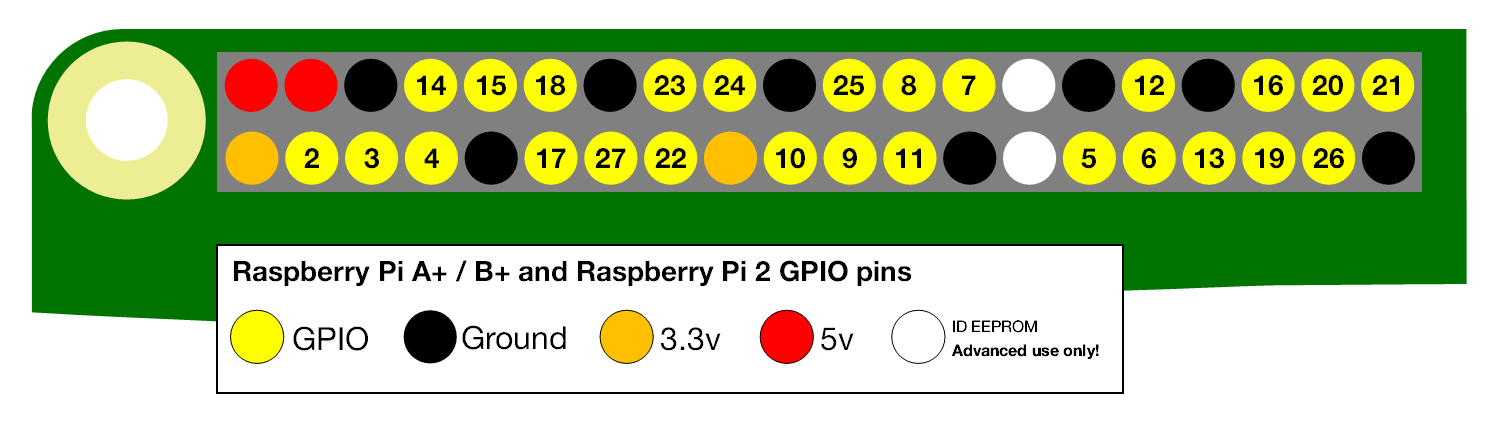
\includegraphics[width=\textwidth]{Bilder/Kapitel2/gpio_pins_pi2.png}
	\caption[Schema GPIO Pins]{Schematische Darstellung der GPIO Pins. Entnommen aus der Raspberry Pi Dokumentation\cite{GPIOMode77:online}.}
	\label{fig:Kapitel2/gpio_pins_pi2.png}
\end{figure}
\noindent
An den vorhandenen 3.3V und 5V Anschlüssen können Sensoren betrieben werden. Dennoch sind nicht alle Sensoren verwendbar. Der Raspberry Pi verfügt nur über die Möglichkeit digitale Signale an den \ac{GPIO} Pins zu verarbeiten. Es werden jedoch neben digitalen auch analoge Sensoren benötigt. Diese können nicht direkt an die Pins angeschlossen werden, aber das Problem ist mit einem \ac{A/D-Wandler} lösbar. \\
Die Erweiterungsplatine RPi-Explorer 700 von Joy-IT \cite{joyitrpi87:online} beinhaltet einen \ac{A/D-Wandler} an dem Analoge Pins angeschlossen werden können. Durch die Erweiterung ist es möglich bis zu vier analoge Sensoren an einem Sensorknoten zu betrieben. \\
Die \ac{GPIO} Schnittstelle unterstützt eine maximale Eingangsspannung von 3.3V, welche für die Sensoren ausreichend ist. Durch die Kompatibilität der Sensoren zum Arduino und dem Raspberry Pi können diese sowohl mit 5V als auch mit 3.3V betrieben werden.
Folgende Sensoren von Allnet\cite{111861pd90:online} werden im \fullref{Verdrahtung_der_Sensoren} verwendet:
\begin{description}
\item[Temperatur und Luftfeuchtigkeitssensor] \hfill \\
	Der Sensor, KY-015, vom Typ DHT11 kann Temperaturen von 0 bis 50$^\circ$C mit einer Messungenauigkeit von $\pm$ 2$^\circ$C messen. Die Luftfeuchtigkeit kann im Bereich von 20 bis 95\% ($\pm$ 5\%) gemessen werden. Hierbei handelt es sich um einen digitalen Sensor.  
\item[Flammensensor]\hfill \\
	Der KY-026 besteht aus einer Fotodiode und einem \ac{Poti}. Die Fotodiode kann Wellenlängen im Bereich von etwa 720 - 1100 nm detektieren. Die Diode hat einen Erfassungswinkel von etwa 60$^\circ$. Der \ac{Poti} wird zur Empfindlichkeitseinstellung genutzt, somit kann eine Reichweite von etwa  ein bis sieben Metern eingestellt werden. Der Sensor besitzt einen "'Digital Out"'-Pin, der high active geschaltet wird. Sobald eine Flamme erkannt wird, liegt eine logische 1 auf dem Pin. Der "'Analog Out"'-Pin liefert ein analoges Signal, an welchem bei einer gemessenen Flamme eine niedrige Spannung anliegt.
\item[Lichtschranke]\hfill \\
	Das KY-010 Modul ist eine Lichtschranke, die beim Unterbrechen eine logische 1 an den digitalen Ausgangspin liefert.
\item[Mikrofon]\hfill \\
	Das Mikrofon, KY-038, hat den gleichen Aufbau wie der Flammensensor. Im Gegensatz zum Flammensensor wird hierbei ein Mikrofonmodul, statt einer Fotodiode genutzt. Die Signale am Digital Out und Analog Out haben die gleiche Funktionalität wie beim Flammensensor. Dieses Modul dient hauptsächlich zur Detektion von kurzen aber lauten Tönen. Ein Anwendungsbeispiel hierfür ist eine Alarmfunktion. Beispielsweise kann das Zerbrechen eines Fensters festgestellt werden.
\item[Lichtsensor]\hfill \\
	Der Lichtsensor KY-018, bestehend aus einem Fotowiderstand, hat bei Dunkelheit einen Widerstand $>$20M$\Omega$ und bei Helligkeit $<$ 80$\Omega$. Damit kann bestimmt werden, ob in einem Zimmer das Licht brennt. Der Lichtsensor liefert ein analoges Signal.
\item[Schocksensor]\hfill \\
	Der Schocksensor liefert eine logische 1 an den Ausgangspin, falls eine Erschütterung festgestellt wurde. Dies dient exemplarisch zur Umsetzung einer Schritterkennung am Boden.
\end{description}

%Harm
\section{WLAN}

%Hacken dran
\subsection{Standard}
Die \ac{IEEE} hat, Mitte der 90er Jahre, den Auftrag bekommen WLAN zu standardisieren. Die Bezeichnung WLAN ist in soweit korrekt, da WLAN in weiten Teilen auf den 802.X Standards basiert, welche Umgangssprachlich als Ethernet bezeichnet werden. Wie aus der \fullref{osi-wlan} hervorgeht, ist der Physical Layer komplett neu erstellt worden und der Data Link Layer erweitert worden. Die restlichen Schichten wurden unverändert übernommen.

\begin{figure} [htb]
\begin{centering}
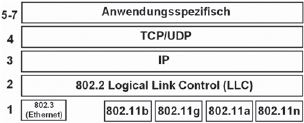
\includegraphics{Bilder/Kapitel2/osi_wlan.jpg}
\caption[WLAN-Protokollstack]{WLAN-Protokollstack \cite{SWB-430171331}}
\label{osi-wlan}
\end{centering}
\end{figure}
\noindent
Die \ac{IEEE} hat 1997 den Standard 802.11 veröffentlicht. Der Standard sieht vor, dass im 2,4 GHz-Band eine Datenrate von 1-2 Mbit/s gewährleistet ist. Im Jahr 1999 wurde der Standard durch 802.11a und 802.11b erweitert. In 802.11a wird vorgesehen, dass im 5 GHz-Band eine Datenrate von 54 Mbit/s möglich ist. Die Erweiterung 802.11b funkt im 2,4 GHz-Band und bietet eine Datenrate von 11 Mbit/s. Im Jahr 2003 ist der Standard um 802.11g erweitert worden. Dieser ermöglicht auch im 2,4 GHz-Band Datenraten von 54 Mbit/s. Im September 2009 ist der Standard 802.11n veröffentlicht worden. Dieser Standard ermöglicht Datenraten von bis zu 150 Mbit/s. Wird 4x4-\ac{MIMO} verwendet sind theoretisch sogar bis zu 600 Mbit/s möglich. Als Frequenzbänder sind sowohl das 2,4 GHz-Band als auch das 5 GHz-Band erlaubt. Im Jahr 2013 ist der Standard 802.11ac veröffentlicht worden. Dieser verwendet nur das 5 GHz-Band, nutzt bis zu 8x8-\ac{MIMO} und ermöglicht Datenraten von bis zu 6,9 Gbit/s. In der \fullref{tab:WLAN-Standards} sind die einzelnen Standards zusammengefasst aufgeführt.

\begin{table}[htb]
\centering
\caption{Übersicht der WLAN-Standards \cite{SWB-430171331}}
\label{tab:WLAN-Standards}
\resizebox{\textwidth}{!}{%
\begin{tabular}{l|l|l|l}
\textbf{WLAN Standard} & \textbf{Veröffentlichungsjahr} & \textbf{Frequenzband}       & \textbf{Theoretische Maximalgeschwindigkeit}  	\\ \hline
802.11        & 1997                  & 2,4 GHz            & 1-2 Mbit/s       											\\ \hline
802.11a       & 1999                  & 5 GHz              & 54 Mbit/s        											\\ \hline
802.11b       & 1999                  & 2,4 GHz            & 11 Mbit/s        											\\ \hline
802.11g       & 2003                  & 2,4 GHz            & 54 Mbit/s        											\\ \hline
802.11n       & 2009                  & 2,4 GHz oder 5 GHz & 150 - 600 Mbit/s 											\\ \hline
802.11ac      & 2013                  & 5 GHz              & 6,9 Gbit/s       											\\ 
\end{tabular}%
}
\end{table} 
\noindent
Der Standard 802.11a ist nicht erfolgreich, da aus Gründen der Rückwärtskompatibilität zu 802.11b/g zwei Frequenzbänder unterstützt werden müssen. Die Unterstützung von beiden Frequenzbändern erhöht die Kosten und die Komplexität. Den Durchbruch erlangte WLAN mit dem Standard 802.11b. Schnellere Internetanbindungen und steigende Anforderungen machten es notwendig mehr Bandbreite zur Verfügung zu stellen. Dies wurde durch den Standard 802.11g realisiert. Da das 2,4 GHz-Band bereits sehr ausgelastet ist und außerdem noch weitere Geräte wie DECT-Funktelefone oder Mikrowellen den Empfang stören können, ist beim Standard 802.11n auch die Nutzung des 5 GHz-Bandes möglich. (vgl. \cite{SWB-430171331})\\

%Hacken dran
\subsubsection{Betriebsmodi von WLAN}
WLAN kann in zwei verschiedenen Modi betrieben werden. Der Ad-Hoc-Modus ist vergleichbar mit einem Crossover-Kabel im Ethernetbereich während der Infrastrukturmodus ähnlich wie ein Switch funktioniert.\\
Beim Ad-Hoc-Modus müssen die beteiligten Benutzer sich über die Einstellungen einigen und diese an ihrem Gerät entsprechend eingeben. Die Kommunikation findet dann direkt zwischen den Endgeräten statt. Andere Geräte können die Datenpakete empfangen, verwerfen diese jedoch, wenn die Zieladresse nicht ihre eigene ist.\\
Der Infrastrukturmodus ist der häufiger anzutreffende Modus. Im Infrastrukturmodus wird das WLAN mit seinen Einstellungen auf einem Access-Point konfiguriert. Ein Anwender kann sich mit diesem Netz unter Angabe der \ac{SSID} und einem eventuell vergebenen Passwort verbinden. Die Verbindung mit einem Access-Point hat den Vorteil, dass ein Gerät erreicht werden kann, welches bei einem Ad-Hoc-Netzwerk zu weit entfernt wäre, um es per Funk zu erreichen. Außerdem muss der Anwender nicht wissen, ob der Kommunikationspartner ein kabelgebundenes Gerät verwendet oder ebenfalls im WLAN zu finden ist. Der Access-Point muss dazu lediglich über ein Kabel an einen Switch angeschlossen sein. (vgl. \cite{SWB-430171331})

%Hacken dran
\subsubsection{Einteilung der Frequenzbänder}
Die Frequenzbänder des 2,4 GHz-Bandes und des 5 GHz-Bandes sind in einzelne Kanäle unterteilt. Das 2,4 GHz-Band ist je nach Land in bis zu 13 Kanäle aufgeteilt, die jeweils eine Breite von 5 MHz haben. Eine Übertragung benötigt jedoch 25 MHz was bedeutet, dass es nur 3 überlappungsfreie Kanäle gibt: Kanal 1, 6 und 11. Im 5 GHz-Band stehen 455 MHz zur Verfügung. Bei einer Übertragung mit 25 MHz ergibt dies 18 mögliche überlappungsfreie Funknetze. Da bei 802.11n und 802.11ac die Übertragung auch 40-160 MHz betragen kann reduziert sich die Anzahl von 18 möglichen Netzen relativ schnell (40 MHz=11 Netze 80MHz=5 Netze 160 MHz=2 Netze). (vgl. \cite{SWB-430171331})

%Hacken dran
\subsubsection{Authentifizierung beim Acces-Point}
Damit ein Endgerät sich mit einem WLAN-Netz verbinden kann, muss es wissen auf welcher Frequenz, in welchem Kanal usw. es arbeitet. Damit dies gewährleistet ist, sendet der Access-Point etwa alle 100 ms ein sogenanntes Beacon aus. In diesem Beacon stecken alle notwendigen Informationen, die ein Client benötigt, um sich mit dem Netz zu verbinden. Nachdem der Client die Einstellungen übernommen hat, sendet er eine Authentifizierungsanfrage an den Access-Point. Diese Anfrage ist keine "`echte"' Authentifizierung, da in der Authentifizierungsanfrage lediglich der Authentifizierungsalgorithmus "`Open"' System mitgeteilt wird. Genügt dem Access-Point diese "`Authentifizierung"', wird diese mit einem positiven Statuscode beantwortet.\\
Im zweiten Schritt wird ein Schlüssel benötigt, der beiden Geräten bekannt ist. Der Access-Point sendet dem Client einen zufälligen Text, den der Client verschlüsselt zurückschicken muss. Entspricht der verschlüsselte Text den Erwartungen, so ist der Client erfolgreich Authentifiziert. (vgl. \cite{SWB-430171331})


%Durch
\subsection{Verschlüsselung}
Da WLAN die Luft als Übertragungsmedium verwendet und jeder darauf zugreifen kann, verdient die Verschlüsselung des Datenverkehrs besondere Aufmerksamkeit. Die Verschlüsselung verhindert, dass Dritte die Kommunikation des Endgeräts mit dem Access-Point mitlesen können. Verschlüsselung hat das Problem, dass beide Geräte ein Geheimnis teilen müssen. Dieses Geheimnis wird Schlüssel genannt. Es gibt aktuell drei Verschlüsselungsverfahren, die verwendet werden können. \ac{WEP} und \ac{WPA}, diese sind bereits geknackt und \ac{WPA2}.
%Durch
\subsubsection{\ac{WEP}}
Die \fullref{wep_funktionsweise} stellt den Verschlüsselungsalgorithmus dar.
Bei der Standardisierung der Standards 802.11b, 802.11g und 802.11a wurde \ac{WEP} integriert. \ac{WEP} basiert auf einem Stream Ciphering-Algorithmus, bei dem die Daten mit einer Ciphersquenz verschlüsselt werden. Die Sequenz wird mit einem \ac{IV} und einem Schlüssel berechnet. Der \ac{IV} ändert sich für jedes Frame und erzeugt somit wechselnde Ciphering Keys. Der daraus berechnete Schlüssel wird mit den Daten der Nachricht durch ein logisches Oder verknüpft. (vgl. \cite{SWB-430171331})


\begin{figure} [htb]
\begin{centering}
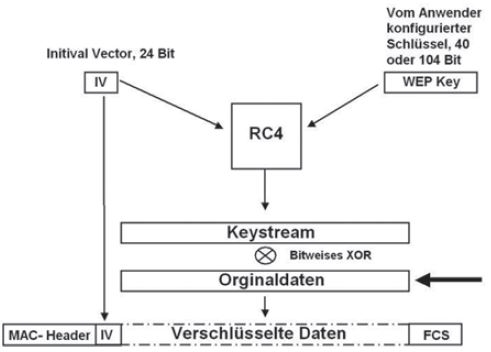
\includegraphics{Bilder/Kapitel2/wep_funktionsweise.jpg}
\caption[WEP-Verschlüsselung]{WEP-Verschlüsselung \cite{SWB-430171331}}
\label{wep_funktionsweise}
\end{centering}
\end{figure}

Problematisch an diesem Verfahren ist, dass der Schlüssel bei jedem Teilnehmer eingetragen werden muss und somit nicht geheim gehalten werden kann. Schwerwiegender ist, dass jedes verschlüsselte Frame am Anfang die gleiche Bytefolge des \ac{LLC}-Headers beinhaltet. Bestimmte \acp{IV} werden im Klartext übertragen, wodurch ein Angreifer nach etwa 5-6 Millionen Paketen den Schlüssel berechnen kann. Mittlerweile sind auch Anwendungen verfügbar, die selbst Datenpakete erzeugen und so in sehr kurzer Zeit, den Schlüssel berechnen können. (vgl. \cite{SWB-430171331})
%TODO: Kann bei Seitenbedarf noch ausgebaut werden
%Durch
\subsubsection{\ac{WPA}} 
Aufgrund der beschriebenen Schwächen von \ac{WEP}, ist 802.11i von der \ac{IEEE} entwickelt worden. Da \ac{WPA2} aber \ac{CCMP} voraussetzt, welches mehr Leistung benötigt, wurde durch die Industrie \ac{WPA} entwickelt. \ac{WPA} funktioniert ebenfalls auf schwächerer Hardware. Als Verschlüsselungsmethode wird \ac{TKIP} und Optional \ac{CCMP} verwendet. Beschrieben wird hier die Funktionsweise mit \ac{TKIP}. \\
\ac{TKIP} verwendet wie \ac{WEP} den RC4-Algorithmus zur Verschlüsselung der Daten aber der Umgang mit Daten und Schlüsseln ist komplexer. \\
Nach \textsc{Klaus Schmeh} \cite{SWB-378541420} ist die Grundlage von \ac{TKIP} der \ac{PMK}, der beiden Seiten bekannt sein muss. Er hat eine Länge von 256 Bit und wird ausschließlich zur Ableitung anderer Schlüssel verwendet. Aus einem \ac{IV}, der MAC-Adresse und dem Daten-Schlüssel wird ein \ac{PPE}-Schlüssel gebildet. Der \ac{PPE}-Schlüssel ist 128 Bit lang und wird für jedes Datenpaket neu generiert.
Der \ac{IV} teilt sich in zwei Teile von denen der erste 16 Bit und der zweite 32 Bit lang ist. Dies ergibt eine Länge von 48 Bit, welche bereits länger als der 24 Bit lange \ac{IV} bei \ac{WEP}ist. Der erste Teil erhöht sich von Paket zu Paket um 1.\\
Wie aus der \fullref{wpa_funktionsweise} hervorgeht, werden der MICHAEL-Schlüssel und die unverschlüsselten Daten an die schlüsselabhängige Hashfunktion MICHAEL übergeben, die einen Hashwert berechnet. Die Daten und der Hashwert werden zusammengefügt und es wird mit \ac{CRC} ein zweiter Hashwert generiert. Verschlüsselt werden die Daten mit den beiden Hashwerten nun mit dem RC4-Verfahren und dem jeweils gültigen \ac{PPE}-Schlüssel. (vgl. \cite{SWB-378541420})

\begin{figure} [htb]
\begin{centering}
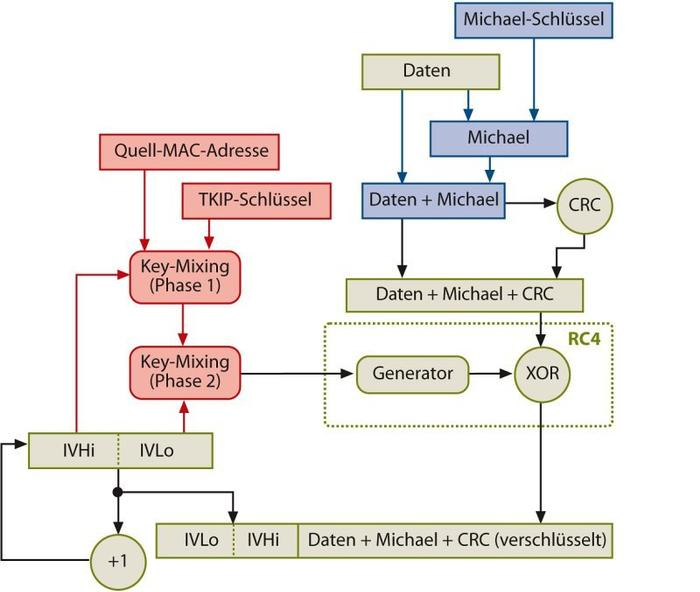
\includegraphics[scale=0.6]{Bilder/Kapitel2/wpa_funktionsweise.jpg}
\caption[WPA-Verschlüsselung]{WPA-Verschlüsselung \cite{Heise-WLAN}}
\label{wpa_funktionsweise}
\end{centering}
\end{figure}
%Durch
\subsubsection{\ac{WPA2}}
\ac{WPA2} und \ac{WPA} sind nahezu identisch. \ac{CCMP} ersetzt \ac{TKIP} und die Hashfunktion MICHAEL. \ac{CCMP} basiert auf dem \ac{AES}-\\
Verschlüsselungsstandard. (vgl. \cite{WPA2})
%TODO: Falls jemand eine Idee hat wie man das noch ausschmücken kann... her damit!!!!